%%%%%%%%%%%%%%%%%%%%%%%%%%%%%%%%%%%%%%%%%%%%%%%%%%%
%
%  New template code for TAMU Theses and Dissertations starting Spring 2018.  
%
%
%  Author: Sean Zachary Roberson
%  Version 3.17.09
%  Last Updated: 9/21/2017
%
%%%%%%%%%%%%%%%%%%%%%%%%%%%%%%%%%%%%%%%%%%%%%%%%%%%

% NOTE: THE ONLY MAJOR CHANGE IS IN THE RELAXATION
% OF MARGIN REQUIREMENTS. THIS TEMPLATE IS THE MOST
% CURRENT. SEE THE FILES README.TXT AND NEWCHANGES.TXT
% FOR MORE INFORMATION.

\documentclass[12pt]{report}

\usepackage{tamuconfig}

% Most of the packages that set the default settings
% for the document have moved to the style file
% tamuconfig.sty. This includes

%These next lines change the font. Fixes for certain
%fonts will be implemented in a future release.

%Comment this line if you do not wish to use Times
%New Roman. The font used will then be the LaTeX
%default of Computer Modern.
\usepackage{times}
%\usepackage{cmbright}
\usepackage[T1]{fontenc}

% For natbib-style references, uncomment this.
%\usepackage{natbib}

%This package allows for the use of graphics in the
%document.
\usepackage{graphicx}
\usepackage{subcaption}
\usepackage{array}

%If you have JPEG format images, add .jpg as an
%allowed file extension below. Same for Bitmaps (.bmp).
\DeclareGraphicsExtensions{.png}

%It is best practice to keep all your pictures in
%one folder inside the main directory in which your
%TeX file is kept. Here the folder is named "graphic."
%Replace the name here with your folder's name, if needed.
%The period is needed due to relative referencing.
\graphicspath{ {./graphic/} }

% For quick document navigation.
\usepackage[hidelinks]{hyperref}

%%%%%%%%%%%%%%%%%%%%%%%%%%%%%%%%%%%%%%%%%%%%%%%%%%%%%%%%%
%Please place all your personal packages here. Check to
%see if the packages you wish to use are not already
%declared above. Placing all your personal packages
%here allows me to determine if there are any package
%issues in compilation, as well as any conflicts
%that may arise by the order of loading.
%--Sean Zachary Roberson
%%%%%%%%%%%%%%%%%%%%%%%%%%%%%%%%%%%%%%%%%%%%%%%%%%%%%%%%%
%%%%%%%%%%%%%%%%%%%%%%%%%%%%%%%%%%%%%%%%%%%%%%%%%%%%%%%%%
%Begin student defined packages.
%%%%%%%%%%%%%%%%%%%%%%%%%%%%%%%%%%%%%%%%%%%%%%%%%%%%%%%%%


%%%%%%%%%%%%%%%%%%%%%%%%%%%%%%%%%%%%%%%%%%%%%%%%%%%%%%%%%
%End student defined packages.
%%%%%%%%%%%%%%%%%%%%%%%%%%%%%%%%%%%%%%%%%%%%%%%%%%%%%%%%%

% End preamble. Document begins below.

\begin{document}

%The title of your document goes here.
%Spacing may need to be adjusted if your title is long
%and pushes the copyright off the page.
\renewcommand{\tamumanuscripttitle}{\textbf{Identification and Resolution of Interpenetration Regions of Woven Fiber Surface Meshes using Different Data Representation Types}}

%Type only Thesis, Dissertation, or Record of Study.
\renewcommand{\tamupapertype}{Thesis Proposal}

%Your full name goes here, as it is in university records. Check your student record on Howdy if there is any mismatch.
\renewcommand{\tamufullname}{Collin Wisenbaker Blake}

%The degree title goes here. See the OGAPS site for more info.
\renewcommand{\tamudegree}{Master of Science}
\renewcommand{\tamuchairone}{Dr. John Whitcomb}


% Uncomment out the next line if you have co-chairs.  You will also need to edit the titlepage.tex file.
%\newcommand{\tamuchairtwo}{Additional Chair Name}
\renewcommand{\tamumemberone}{Dr. Darren Hartl}
\newcommand{\tamumembertwo}{Dr. Terry Creasy}
%\newcommand{\tamumemberthree}{Committee Member 3}
\renewcommand{\tamudepthead}{Dr. Rodney Bowersox}

%Type only May, August, or December.
\renewcommand{\tamugradmonth}{August}
\renewcommand{\tamugradyear}{2018}
%Your department name goes here.
\renewcommand{\tamudepartment}{Aerospace Engineering}


%%%%%%%%%%%%%%%%%%%%%%%%%%%%%%%%%%%%%%%%%%%%%%%%%%%
%
%  New template code for TAMU Theses and Dissertations starting Fall 2016.  
%
%
%  Author: Sean Zachary Roberson
%  Version 3.17.09
%  Last Updated: 9/21/2017
%
%%%%%%%%%%%%%%%%%%%%%%%%%%%%%%%%%%%%%%%%%%%%%%%%%%%

%%%%%%%%%%%%%%%%%%%%%%%%%%%%%% 
%% TITLE PAGE
%% The values get updated automatically.  Please do not make changes to this file other than adding/deleting committee members where necessary.
%%%%%%%%%%%%%%%%%%%%%%%%%%%%%%

\providecommand{\tabularnewline}{\\}



\begin{titlepage}
\begin{center}
\MakeUppercase{\tamumanuscripttitle}
\vspace{4em}

A \tamupapertype

by

\MakeUppercase{\tamufullname}

\vspace{4em}

\begin{singlespace}

Submitted to the Office of Graduate and Professional Studies of \\
Texas A\&M University \\

in partial fulfillment of the requirements for the degree of \\
\end{singlespace}

\MakeUppercase{\tamudegree}
\par\end{center}
\vspace{2em}
\begin{singlespace}
\begin{tabular}{ll}
 & \tabularnewline
& \cr
% If you have Co-Chairs comment out the 'Chair of Committee' line below and uncomment the 'Co-Chairs of Committee' line.
Chair of Committee, & \tamuchairone\tabularnewline
%Co-Chairs of Committee, & \tamuchairone\tabularnewline & \tamuchairtwo\tabularnewline
Committee Members, & \tamumemberone\tabularnewline
 & \tamumembertwo\tabularnewline
Head of Department, & \tamudepthead\tabularnewline

\end{tabular}
\end{singlespace}
\vspace{3em}

\begin{center}
\tamugradmonth \hspace{2pt} \tamugradyear

\vspace{3em}

Major Subject: \tamudepartment \par
\vspace{3em}
Copyright \tamugradyear \hspace{.5em}\tamufullname 
\par\end{center}
\end{titlepage}
\pagebreak{}




 % This is simply a file that formats and adds your titlepage, please do not edit this unless you have a specific need. .
%%%%%%%%%%%%%%%%%%%%%%%%%%%%%%%%%%%%%%%%%%%%%%%%%%%
%
%  New template code for TAMU Theses and Dissertations starting Fall 2016.  
%
%
%  Author: Sean Zachary Roberson
%  Version 3.17.09
%  Last Updated: 9/21/2017
%
%%%%%%%%%%%%%%%%%%%%%%%%%%%%%%%%%%%%%%%%%%%%%%%%%%%
%%%%%%%%%%%%%%%%%%%%%%%%%%%%%%%%%%%%%%%%%%%%%%%%%%%%%%%%%%%%%%%%%%%%%
%%                           ABSTRACT 
%%%%%%%%%%%%%%%%%%%%%%%%%%%%%%%%%%%%%%%%%%%%%%%%%%%%%%%%%%%%%%%%%%%%%

\chapter*{ABSTRACT}
\addcontentsline{toc}{chapter}{ABSTRACT} % Needs to be set to part, so the TOC doesnt add 'CHAPTER ' prefix in the TOC.

\pagestyle{plain} % No headers, just page numbers
\pagenumbering{roman} % Roman numerals
\setcounter{page}{2}

As the usage of computational analysis for composite design becomes increasingly more popular, the desire to create and test textile composite materials is increasing as well. Previous research and study has been conducted using idealized woven textile geometries that lack the realism of imperfect woven composite fiber bundles (or tows). For most analyses, a filament (bundles of fibers) discretization of the tow is too complex to be analyzed, so instead, a surface representation of the tows is created so that homogenized properties can be applied. This representation is an approximation of the fiberized tow. When theses surfaces are created, small regions of inter-penetrations are formed where the surfaces cross into each other. This creates two problems: a physically impossible occupation of the same space concerning the tows and incompatibility of the mesh resulting from these meshes crossing through each other.


This research proposal will outline a plan to address these problems and resolve them. The following three objectives are proposed rectify this issue: (1) Distinguish between data types that can be used to define the surface geometry, (2) Identify the regions of inter-penetrations between the surfaces, and (3) Discuss resolution to the interpenetration regions. The results of this study could result in more realistic woven textile geometries for computational testing of these complex composites that are compatible with traditional finite element analysis.


 

\pagebreak{}

%%%%%%%%%%%%%%%%%%%%%%%%%%%%%%%%%%%%%%%%%%%%%%%%%%%
%
%  New template code for TAMU Theses and Dissertations starting Fall 2016.  
%
%
%  Author: Sean Zachary Roberson
%  Version 3.17.09
%  Last Updated: 9/21/2017
%
%%%%%%%%%%%%%%%%%%%%%%%%%%%%%%%%%%%%%%%%%%%%%%%%%%%


%%%%%%%%%%%%%%%%%%%%%%%%%%%%%%%%%%%%%%%%%%%%%%%%%%%%%%%%%%%%%%%%%%%%%%
%%             CONTRIBUTORS AND FUNDING SOURCES
%%%%%%%%%%%%%%%%%%%%%%%%%%%%%%%%%%%%%%%%%%%%%%%%%%%%%%%%%%%%%%%%%%%%%
\chapter*{CONTRIBUTORS AND FUNDING SOURCES}
\addcontentsline{toc}{chapter}{CONTRIBUTORS AND FUNDING SOURCES}  % Needs to be set to part, so the TOC doesn't add 'CHAPTER ' prefix in the TOC.


%This section is taken directly from the MS Word templates.

%Old version below.

%All theses and dissertations must include a contributors and funding sources section. In this section, name all members of the dissertation committee, and any collaboration with others in carrying out your thesis or dissertation research. Your independent contributions must be made clear.
%
%If financial support from the university or any other source was gained to conduct your thesis or dissertation research and compilation, it must be listed in this section. If you completed all work independently without outside financial support, indicate this here.
%\textit{(Sample Wording)}
%
%This work was supported by a dissertation committee consisting of Professor XXX [advisor – also note if co-advisor] and XXXX of the Department of [Home Department] and Professor(s) XXXX of the Department of [Outside Department].
% 
%The data analyzed for Chapter III was provided by Professor XXXX. The analyses depicted in Chapter IV were conducted in part by Rebecca Jones of the Department of Biostatistics and were published in (year) in an article listed in the Biographical Sketch. 
%
%All other work conducted for the dissertation was completed by the student independently.
%
%\noindent \textit{(or)}
%
%This work was supervised by a dissertation committee consisting of Professor XXXX [advisor – also note if co-advisor] and Professor(s) XXXX of the Department of [Home Department] and Professor(s) XXXX of [Outside Department]. All work for the dissertation was completed independently by the student.
%
%\noindent \textit{(or)}
%
%Graduate study was supported by a fellowship from Texas A\&M University and a dissertation research fellowship from XXX Foundation.

\subsection*{Contributors}
This work was supported by a thesis committee consisting of Dr. John Whitcomb and Dr. Darren Hartl of the Department of Aerospace Engineering and Dr. Terry Creasy of the Department of Materials Science and Engineering.

%A computational library was extensively used and was written by the Geometry Group at SINTEF ICT, Department of Applied Mathematics. An existing framework for finite element meshes was also used and was developed by **NAME**.

All other work conducted for the thesis was completed by the student independently.
\subsection*{Funding Sources}
**Ask Dr. Whitcomb** 
\pagebreak{}
%%%%%%%%%%%%%%%%%%%%%%%%%%%%%%%%%%%%%%%%%%%%%%%%%%%
%
%  New template code for TAMU Theses and Dissertations starting Fall 2016.  
%
%
%  Author: Sean Zachary Roberson
%  Version 3.17.09
%  Last Updated: 9/21/2017
%
%%%%%%%%%%%%%%%%%%%%%%%%%%%%%%%%%%%%%%%%%%%%%%%%%%%

%%%%%%%%%%%%%%%%%%%%%%%%%%%%%%%%%%%%%%%%%%%%%%%%%%%%%%%%%%%%%%%%%%%%%%
%%                           NOMENCLATURE
%%%%%%%%%%%%%%%%%%%%%%%%%%%%%%%%%%%%%%%%%%%%%%%%%%%%%%%%%%%%%%%%%%%%%

\chapter*{NOMENCLATURE}
\addcontentsline{toc}{chapter}{NOMENCLATURE}  % Needs to be set to part, so the TOC doesnt add 'CHAPTER ' prefix in the TOC.

%A note about aligning: These entries will align
%themselves according to the ampersand (&).
%No extra spaces are needed, as seen in some of
%the entries below.

%Example of the longtable environment.
\hspace*{-1.25in}
\vspace{12pt}
\begin{spacing}{1.0}
	\begin{longtable}[htbp]{@{}p{0.35\textwidth} p{0.62\textwidth}@{}}
	   % \begin{tabular}{@{}p{0.33\textwidth} p{0.62\textwidth}@{}}
		TAMU			&	Texas A\&M University\\	[2ex]
		VTMS & Virtual Textile Morphology Suite\\ [2ex]
%		SISL & Non-Uniform Rational B-Spline Library\\ [2ex]
%		NURBS & Non-Uniform Rational B-Splines \\ [2ex]
		AFRL & Air Force Research Lab in Dayton, Ohio\\ [2ex]
		FEA & Finite Element Analysis \\ [2ex]
		%XXXXXXXX		&	This is an optional page. Random word to test how long the sentence can be? This is just for test purpose. The current setting aims to align left/right margin same as all other pages.\\	[2ex]
	   % \end{tabular}%
	\end{longtable}
\end{spacing}

\pagebreak{}

%%%%%%%%%%%%%%%%%%%%%%%%%%%%%%%%%%%%%%%%%%%%%%%%%%%
%
%  New template code for TAMU Theses and Dissertations starting Fall 2016.  
%
%
%  Author: Sean Zachary Roberson
%  Version 3.17.09
%  Last Updated: 9/21/2017
%
%%%%%%%%%%%%%%%%%%%%%%%%%%%%%%%%%%%%%%%%%%%%%%%%%%%
%%%%%%%%%%%%%%%%%%%%%%%%%%%%%%%%%%%%%%%%%%%%%%%%%%%%%%%%%%%%%%%%%%%%%%
%%       TABLE OF CONTENTS
%%%%%%%%%%%%%%%%%%%%%%%%%%%%%%%%%%%%%%%%%%%%%%%%%%%%%%%%%%%%%%%%%%%%%
% single-space sections in Table of Contents  - commented in version 1.7
%\renewcommand{\cftsecafterpnum}{\vskip0.5\baselineskip}
%\renewcommand{\cftsubsecafterpnum}{\vskip0.5\baselineskip}
%\renewcommand{\cftsubsubsecafterpnum}{\vskip0.5\baselineskip}
%%%%%%%%%%%%%%%%%%%%%%%%%%%%%%%%%%%%%%%%%%%%%%%%%%%

\phantomsection
\addcontentsline{toc}{chapter}{TABLE OF CONTENTS}  

\begin{singlespace}
\renewcommand\contentsname{\normalfont} {\centerline{TABLE OF CONTENTS}}

\setcounter{tocdepth}{4} % This puts \subsubsection[]{×} in your List of Tables.  The default is 3.


%%%%%%%%%%%%%  Adds Page above the page number in TOC
\setlength{\cftaftertoctitleskip}{1em}
\renewcommand{\cftaftertoctitle}{%
\hfill{\normalfont {Page}\par}}


\tableofcontents

%\addtocontents{toc}{\protect\afterpage{~\hfill\normalfont{Page}\par\medskip}}
\end{singlespace}

\pagebreak{}

%%%%%%%%%%%%%%%%%%%%%%%%%%%%%%%%%%%%%%%%%%%%%%%%%%%%%%%%%%%%%%%%%%%%%%
%%                           LIST OF FIGURES
%%%%%%%%%%%%%%%%%%%%%%%%%%%%%%%%%%%%%%%%%%%%%%%%%%%%%%%%%%%%%%%%%%%%%

\phantomsection
\addcontentsline{toc}{chapter}{LIST OF FIGURES}  

\renewcommand{\cftloftitlefont}{\center\normalfont\MakeUppercase}

\setlength{\cftbeforeloftitleskip}{-12pt} %% Positions the LOF title vertically to match the chapter titles
\renewcommand{\cftafterloftitleskip}{12pt}


\renewcommand{\cftafterloftitle}{%
\\[4em]\mbox{}\hspace{2pt}FIGURE\hfill{\normalfont Page}\vskip\baselineskip}

\begingroup


\begin{center}
\begin{singlespace}
%% These values make the lof table entries appear double spaced between.
\setlength{\cftbeforechapskip}{0.4cm}
\setlength{\cftbeforesecskip}{0.30cm}
\setlength{\cftbeforesubsecskip}{0.30cm}
\setlength{\cftbeforefigskip}{0.4cm}
\setlength{\cftbeforetabskip}{0.4cm}

% Provided by Andy Philips.
% needed to make chapter gaps look no different than sections:
% \addtocontents{lof}{\protect\renewcommand*\protect\addvspace[1]{}}

% Philips' document had 30 figures. Is there a maximum number of figures
% that changes the spacing to non-uniform, i.e., not double-spaced
% between all entries?

\listoffigures

\end{singlespace}
\end{center}

\pagebreak{}


%%%%%%%%%%%%%%%%%%%%%%%%%%%%%%%%%%%%%%%%%%%%%%%%%%%%%%%%%%%%%%%%%%%%%%
%%                           LIST OF TABLES
%%%%%%%%%%%%%%%%%%%%%%%%%%%%%%%%%%%%%%%%%%%%%%%%%%%%%%%%%%%%%%%%%%%%%%
%
\phantomsection
\addcontentsline{toc}{chapter}{LIST OF TABLES}  

\renewcommand{\cftlottitlefont}{\center\normalfont\MakeUppercase}

\setlength{\cftbeforelottitleskip}{-12pt} %% Positions the LOT title vertically to match the chapter titles

%Note that the similar parameter in the LOF is 12pt; this
%is intentional to make the spacing between the headers
%and the first entry look consistent.
\renewcommand{\cftafterlottitleskip}{1pt}


\renewcommand{\cftafterlottitle}{%
\\[4em]\mbox{}\hspace{2pt}TABLE\hfill{\normalfont Page}\vskip\baselineskip}

\begin{center}
\begin{singlespace}

%% These values make the lot table entries appear double spaced between.
\setlength{\cftbeforechapskip}{0.4cm}
\setlength{\cftbeforesecskip}{0.30cm}
\setlength{\cftbeforesubsecskip}{0.30cm}
\setlength{\cftbeforefigskip}{0.4cm}
\setlength{\cftbeforetabskip}{0.4cm}

\listoftables 

\end{singlespace}
\end{center}
\endgroup
\pagebreak{}  % Need this for the pagenumbering to be correct.   % This is simply a file that formats and adds your toc, lof, and lot, please do not edit this unless you have a specific need.

%%%%%%%%%%%%%%%%%%%%%%%%%%%%%%%%%%%%%%%%%%%%%%%%%%%
%
%  New template code for TAMU Theses and Dissertations starting Fall 2016.  
%
%
%  Author: Sean Zachary Roberson
%  Version 3.17.09
%  Last Updated: 9/21/2017
%
%%%%%%%%%%%%%%%%%%%%%%%%%%%%%%%%%%%%%%%%%%%%%%%%%%%

%%%%%%%%%%%%%%%%%%%%%%%%%%%%%%%%%%%%%%%%%%%%%%%%%%%%%%%%%%%%%%%%%%%%%%
%%                           SECTION I
%%%%%%%%%%%%%%%%%%%%%%%%%%%%%%%%%%%%%%%%%%%%%%%%%%%%%%%%%%%%%%%%%%%%%


\pagestyle{plain} % No headers, just page numbers
\pagenumbering{arabic} % Arabic numerals
\setcounter{page}{1}


\chapter{\uppercase {Introduction and Literature Review}}

 The growing use of fiber-matrix composite materials as both a decorative and functional material has also increased the need to better understand these materials in all of their forms. From unidirectional ply composites to intricate woven textile composites, the need for understanding material properties and mechanics for these composites has never been higher. In order to gain a more intimate understanding of the mechanical response for these composites, research turned towards computational models and simulations that were validated with experimental data. As these models became more accurate, understanding of both mechanical response and damage initiation increased. The use of computational models and analysis is now a fundamental aspect of most engineering and scientific research, and can been seen in use as far as early undergraduate studies.


\section{Motivation}

The motivation for this work comes from the desire to more correctly and realistically model fiber-matrix composite materials. Substantial experimental and computational research has been conducted on unidirectional ply composite as well as experimental research on textile woven composites. However, there is still a need for non-idealized textile composite geometries for computational analysis. The use of these geometries range from verification of computational models to insight into damage initiation and growth. 

While there exists multiple software that can generate these geometries, the process (to be discussed later) can result is surface meshes of the geometries can be incompatible and have inter-penetrations between them. A generalized solution to this issue could prove useful to future research in this area.

\section{Woven Textile Composite Simulation}

One method to creating more realistic woven geometries is to simulate the process that manufactures employ to create the fabrics \cite{Wang_Sun1}. The process begins by simulating bundles of fibers as "yarns". These yarns  are made up of digital elements (cylindrical bars connected by friction-less pins) chained together. Each bar is given a stiffness in the longitudinal direction that amounts to a large value which eliminates yarn stretching. Then, a finite element style contact problem is solved where pins between two yarns can create contact forces between each other as well as friction forces. The result is realistic interactions between the digital chains. \cite{Wang_Sun1} 

The result is fiber bundle cross sections that are similar to micro-CT scans from actual woven specimens, shown in Figure 1.1, from \cite{Wang_Sun1}.

\begin{figure}[ht]
\centering
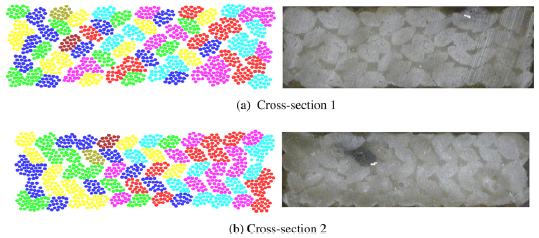
\includegraphics[scale=0.95]{CrossSections.png}
\caption[Simulated vs. Actual Fiber Bundle Cross Sections]{Simulated (left (a) and (b)) vs. Actual Fiber Bundle Cross Sections}

\end{figure}


While there is possibly other software that can accomplish this level of similarity between simulation and reality, only two were explored. The first is Digital Fabric Mechanics Analyzer (DFMA) from Kansas State, overseen by Youqi Wang and students. The other is Virtual Textile Morphology Suite (VTMS), developed by Eric Zhou at AFRL. It should be noted that Eric Zhou is a former student of Youqi Wang and is cited in a previous paper \cite{Wang_Zhou1}.

It is from VTMS that the base geometry and surface mesh that is used in this study originates. Figure 1.2 shows the process visually. The surface inter-penetrations come as a result from the geometries shown in Figure 1.2.d).

\begin{figure}
\centering
\begin{subfigure}{.45\textwidth}
  \centering
  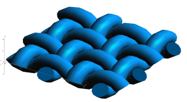
\includegraphics[width=.8\linewidth]{VTMS_Tubes.png}
  \caption{Generic Approximation of Woven Pattern}
\end{subfigure}
\begin{subfigure}{.45\textwidth}
  \centering
  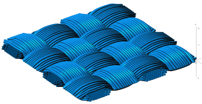
\includegraphics[width=.8\linewidth]{VTMS_Textile.png}
  \caption{Yarn Representation of Pattern}
\end{subfigure}

\begin{subfigure}{.45\textwidth}
  \centering
  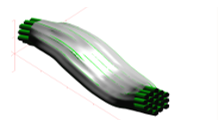
\includegraphics[width=.8\linewidth]{VTMS_Wrapped.png}
  \caption{Surface Approximation of Yarn Bundles}
\end{subfigure}
\begin{subfigure}{.45\textwidth}
  \centering
  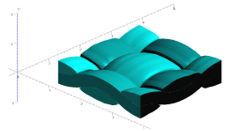
\includegraphics[width=.8\linewidth]{VTMS_Surface.png}
  \caption{Volume Model Derived from Surfaces}
\end{subfigure}
\caption{Evolution of Weave Textile Geometry}
\end{figure}

The reasoning behind creating surface and volume approximations (Figure 1.2.c and d) is that the computational cost of analyzing many bundles that represent woven fibers is very high. Instead, researchers currently are content with using a surface or volume approximation and applying material properties found in experiments.

\section{Introduction to Interpenetration Regions}

Once a surface representation is created, surfaces in close proximity have the ability to penetrate into each other, as shown in Figure 1.3. The arrows in Figure 1.3.b) indicate regions where one surface mesh is penetrating into the other. Physically, the two surfaces would come into contact and create some form of surface. This reaction is not represented here because the surfaces are created after the simulation process is done. These inter-penetrations represent the error in approximating the yarn bundles as a surface to apply homogenized properties to for analysis. Here in lies the focus of this study. Traditional finite element software requires that two geometries can not occupy the same space and must have compatible meshes along any boundaries that they may share. These regions must be fixed if a traditional FEA is to be conducted.

\begin{figure}[H]
\centering
\begin{subfigure}{.6\textwidth}
  \centering
  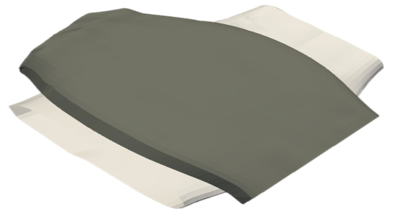
\includegraphics[width=.8\linewidth]{Close_Tows.png}
  \caption{Two Tow Surfaces in Close Proximity}
\end{subfigure}

\begin{subfigure}{.6\textwidth}
  \centering
  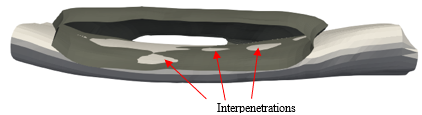
\includegraphics[width=.8\linewidth]{Penetrating_Tows.png}
  \caption{Through View of Penetrating Tows}
\end{subfigure}
\caption{Tow Surface Illustration and Penetrations}
\label{fig:fig}
\end{figure}

\section{VTMS Surface Representation Types}

VTMS has two distinct data types for its surface representations. They will be discussed below.
\subsection*{VTMS' Standard Tow Format}
Once the yarn bundles are approximated as a surface, VTMS stores this surface as a standard tow format. Internally in the software, this data structure stores surface node coordinates and normals, along with stacks that define the cross-section of the surface along the tow path. Also internally stored are surface elements that connect surface nodes and are used for visualization purposes. However, once this data is exported to a file, only node location, node normal, and which stack the nodes belong to is stored. This effectively reduces the usefulness of the data when exported. 

\subsection*{VTMS' Clipped Tow Format}
Once the surface representations in VTMS are clipped to a desired dimension, the surface data is transformed into the clipped tow format. The clipped tow format is similar to many finite element mesh representations. When exported to a file, the data is organized into node location information, surface element type, and the connectivity of the surface elements by referencing node number. The file also stores the outward normal of each surface element. The internal representation of this data is similar to the exported representation and there is much less information lost when exported. 



%%%%%%%%%%%%%%%%%%%%%%%%%%%%%%%%%%%%%%%%%%%%%%%%%%%
%
%  New template code for TAMU Theses and Dissertations starting Fall 2016.  
%
%
%  Author: Sean Zachary Roberson
%  Version 3.17.09
%  Last Updated: 9/21/2017
%
%%%%%%%%%%%%%%%%%%%%%%%%%%%%%%%%%%%%%%%%%%%%%%%%%%%

%%%%%%%%%%%%%%%%%%%%%%%%%%%%%%%%%%%%%%%%%%%%%%%%%%%%%%%%%%%%%%%%%%%%%%%
%%%                           SECTION II
%%%%%%%%%%%%%%%%%%%%%%%%%%%%%%%%%%%%%%%%%%%%%%%%%%%%%%%%%%%%%%%%%%%%%%


\chapter{RESEARCH OBJECTIVES}

To guide this study, three main goals were established to be completed during the duration of this research. These objectives will be discussed regarding both the result of completion and the foreseeable method. They are as follows:
\begin{enumerate}
\item Determine data representation types that will best describe the geometries from VTMS.
\item Implement methods for each representation type that will accurately identify interpenetration regions.
\item Discuss and implement methods that resolve inter-penetrations for each representation type.
\end{enumerate}

\section{Surface Representation Data Types}
There are many types of computational analyses that can be used on computer models and geometries. Inherently, there are also many ways to describe this data. The first objective will be to explore possible representations of the data from VTMS and how they relate to the default types given from this software. This objective is a prerequisite to the remaining objectives as it is important to use the best suited data type for identifying and resolving inter-penetration regions between surfaces.

The origin software VTMS is written in C++ and it is the goal of this study to create a set of software that can implemented in not just VTMS but other software as well. Therefore, the methods developed will be written in C++. Completion of this objective will allow for a easy to use software that can translate  the representation of the geometries in VTMS to other representation types.

\section{Identification of Interpenetration Regions}

The second objective will determine an accurate way to identify inter-penetration regions for the representation types chosen in the first objective. It is important that the detection algorithm correctly identify the regions inter-penetrating so that all incompatibilities may be fixed. The results of completing this objective will given all the information needed to correctly fix the inter-penetrations for the respective representation type for the geometries. 

\section{Resolution of Interpenetration Regions}

The third objective is to identify a method that can resolve the issue of inter-penetrations for each representation type identified in the first objective. Once the method is identified, it will be implemented if possible or the required data to solve the inter-penetration will be given to the user. This will allow for multiple possible solutions to be implemented. It is conceivable that some solutions may be too complex to be implemented during this study.

%%%%%%%%%%%%%%%%%%%%%%%%%%%%%%%%%%%%%%%%%%%%%%%%%%%
%
%  New template code for TAMU Theses and Dissertations starting Fall 2016.  
%
%
%  Author: Sean Zachary Roberson
%  Version 3.17.09
%  Last Updated: 9/21/2017
%
%%%%%%%%%%%%%%%%%%%%%%%%%%%%%%%%%%%%%%%%%%%%%%%%%%%
%%%%%%%%%%%%%%%%%%%%%%%%%%%%%%%%%%%%%%%%%%%%%%%%%%%%%%%%%%%%%%%%%%%%%%
%%                           SECTION III
%%%%%%%%%%%%%%%%%%%%%%%%%%%%%%%%%%%%%%%%%%%%%%%%%%%%%%%%%%%%%%%%%%%%%

\chapter{Proposed Methods}

The following chapter will discuss an approach to each of the previous discussed research objectives.
\section{Surface Representation Data Types}

Although the specific problem presented in this research may be fairly new, detecting collisions and conducting object intersection detection is not. Therefore, a review will be performed on current and antiquated techniques for solving these problems and the representation of the data that describes the objects being used in these methods. Two sources of inspiration that will be heavily explored is the video gaming industry and the computer-aided design (CAD) industry.

Many video games today have three dimensional worlds where the user can often run into and jump onto objects that occupy the world space. These video games conducting hundreds of collision detection tests a minute. Therefore, a study into how they represent the objects that can interact and how they detect these intersections will be conducted. It stands that any method used in this industry will be computationally efficient as collisions in many video game titles happen in fractions of a second.

Computer-aided design software (such as Auto Cad\textsuperscript{\textregistered} and Solidworks\textsuperscript{\textregistered}) have the ability to subtract volumes from each other and highlight intersection boundaries. They can do this very accurately for parts that must fit together with small tolerances. The method in which they both describe their parts and detect these intersections could be very influential in the surface representation type used in detecting and solving the inter-penetrations discussed in this research. A study into the theory of how these types of software are able to accurately describe these intersections will also be conducted. 

An ideal data type to be used for identification and resolution of inter-penetrations will be directly related to the data either internally stored or exported from VTMS. Any data type chosen for the remaining objectives should not overly modify or approximate the data given from VTMS. Ease of implementation and use of data types will also influence which representation types are explored. A representation that helps identify and resolve inter-penetrations accurately and in a timely manner is the goal of this objective.

A preliminary study into both of these areas revealed that most video games make use of a surface polygon mesh of objects. \cite{Bobic,Souto}. CAD programs can use implicit and parametric representations of surfaces that make up the three dimensional objects that can collide \cite{CAD}.

\section{Identification of Interpenetration Regions}

The exact method for accurately identifying inter-penetrating regions between surface representations will depend on the chosen representation types. From the preliminary study mentioned previously, one representation type is a polygon surface description that has use in the video game industry. In \cite{Bobic, Souto}, different methods for avoiding and identifying inter-penetrations are discussed. Some of these ideas may be adapted for the purposes of this research.

Another potential type of representation of the tow surfaces is an analytical surface. Rather, a surface that can be defined by a single or set of equations. This readily seen in CAD software design \cite{CAD}. In these types of software, there are algorithms that are used to define where two bodies intersect. These algorithms also may be adapted for the needs of this study.

\section{Resolution of Interpenetration Regions}

Similar to the detection of inter-penetrations, the resolution of inter-penetrations will also depend on the representation type used to describe the tow surfaces. The representations discovered thus far have been accompanied with a standard form of a solution. Therefore, the process of solving the inter-penetrations will conceivably consist of methods adapted from the standard solution form. In each case of representation type, the solution will be adapted and implemented for this research.
%%%%%%%%%%%%%%%%%%%%%%%%%%%%%%%%%%%%%%%%%%%%%%%%%%%
%
%  New template code for TAMU Theses and Dissertations starting Fall 2016.  
%
%
%  Author: Sean Zachary Roberson
%  Version 3.17.09
%  Last Updated: 9/21/2017
%
%%%%%%%%%%%%%%%%%%%%%%%%%%%%%%%%%%%%%%%%%%%%%%%%%%%
%%%%%%%%%%%%%%%%%%%%%%%%%%%%%%%%%%%%%%%%%%%%%%%%%%%%%%%%%%%%%%%%%%%%%%
%%                           SECTION IV
%%%%%%%%%%%%%%%%%%%%%%%%%%%%%%%%%%%%%%%%%%%%%%%%%%%%%%%%%%%%%%%%%%%%%



\chapter{EXPECTED RESULTS}
The following are the expected results for each objective of this research.
\section{Surface Representation Data Types}

Multiple types of representation are expected to be found during this objective. The purpose of this objective is to identify ideal representation types that will aid in fulfilling the remaining objectives.

The results from this objective are expected to be:

\begin{itemize}
	\item One or more surface representation types that can be used to describe the data from VTMS
	\item Insight into conventions of multiple industries that use penetration and collision detection algorithms
	\item Inspiration on multiple types of identification and resolution methods
\end{itemize}

\section{Identification of Interpenetration Regions}

Properly identifying the inter-penetration regions of the surface representations is vital to completing the third object of this research. Without proper identification, there can not be a complete resolution of the inter-penetration regions.

The results from this objective are expected to be:
\begin{itemize}
	\item An algorithm that accurately detects inter-penetration regions for multiple representation types
	\item An algorithm that collects the required data to resolve inter-penetrations
	\item A methodology to accurately visualize interpenetration regions
\end{itemize}

\section{Resolution of Interpenetration Regions}

Completion of this research is synonymous with resolving inter-penetrations or determining the remaining steps for the most realistic solution. The best solution to resolving these inter-penetrations may vary depending on the situation.

The results from this objective are expected to be:
\begin{itemize}
	\item An algorithm that resolves inter-penetrations for one or more of the chosen representation types
	\item Recommendations for the usage of algorithms and methods developed during this research
	\item A method that exports useful inter-penetration data for user discretion
	\item A suite of software that can be easily implemented for other users
\end{itemize}


%%%%%%%%%%%%%%%%%%%%%%%%%%%%%%%%%%%%%%%%%%%%%%%%%%%
%
%  New template code for TAMU Theses and Dissertations starting Fall 2016.  
%
%
%  Author: Sean Zachary Roberson
%  Version 3.17.09
%  Last Updated: 9/21/2017
%
%%%%%%%%%%%%%%%%%%%%%%%%%%%%%%%%%%%%%%%%%%%%%%%%%%%
%%%%%%%%%%%%%%%%%%%%%%%%%%%%%%%%%%%%%%%%%%%%%%%%%%%%%%%%%%%%%%%%%%%%%%
%%                           SECTION V
%%%%%%%%%%%%%%%%%%%%%%%%%%%%%%%%%%%%%%%%%%%%%%%%%%%%%%%%%%%%%%%%%%%%%



\chapter{RESEARCH PLAN}

\section{Time-line}

Below is a time-line that breaks down each object into work done by each academic semester.

\begin{table}[!htb]

\centering
\caption[Research Timeline By Semester]{Research Timeline By Semester}
\begin{tabular}{|>{\centering\arraybackslash}m{3.7cm}||>{\centering\arraybackslash}m{3.7cm}|>{\centering\arraybackslash}m{3.7cm}|>{\centering\arraybackslash}m{3.7cm}|}
\hline
\textbf{Objective} & \textbf{Spring 2017} & \textbf{Fall 2017} & \textbf{Spring 2018} \\ \hline \hline
\textbf{\textit{Surface Representation Data Types}} & Literature Review and Determination of Data Types &  &  \\ \hline
\textbf{\textit{Identification of Interpenetration Region}} &  Literature Review and Discovery of Methods & Implementation of Methods & Use of Methods \\ \hline
\textbf{\textit{Resolution of Interpenetration Region}} & & Literature Review and Planning of Methods & Implementation and Verification of Methods \\ \hline

\end{tabular}
\end{table}

\section{Resources and Equipment}

This research is entirely digital and requires no physical equipment apart from a computer. The software will be developed in C++ which requires a compiler and editing software. It is also likely that external software libraries not developed by the student and will be noted.



%The next line is the format for inserting new sections.
%Replace the name "newsection"  with the name of your
%new section file.
%\include{data/newsection}

%fix spacing in bibliography, if any...
%%%%%%%%%%%%%%%%%%%%%%%%%%%%%%%%%%%%%%%%%%%%%%%%%%%%%%%%%%%%%
\let\oldbibitem\bibitem
\renewcommand{\bibitem}{\setlength{\itemsep}{0pt}\oldbibitem}
%%%%%%%%%%%%%%%%%%%%%%%%%%%%%%%%%%%%%%%%%%%%%%%%%%%%%%%%%%%%%%%
%The bibliography style declared is the IEEE format. If
%you require a different style, see the document
%bibstyles.pdf included in this package. This file,
%hosted by the University of Vienna, shows several
%bibliography styles and examples of in-text citation
%and a references page.
\bibliographystyle{ieeetr}

\phantomsection
\addcontentsline{toc}{chapter}{REFERENCES}

\renewcommand{\bibname}{{\normalsize\rm REFERENCES}}

%This file is a .bib database that contains the sources.
%This removes the dependency on the previous file
%bibliography.tex.
\bibliography{data/myReferences}




%This next line includes appendices. The file
%appendix.tex contains commands pointing to
%the appendix files; be sure to change these
%pointers if you end up changing the filenames.
%Leave this commented if you will not need
%appendix material.
%%%%%%%%%%%%%%%%%%%%%%%%%%%%%%%%%%%%%%%%%%%%%%%%%%%%
%
%  New template code for TAMU Theses and Dissertations starting Fall 2016.  
%
%
%  Author: Sean Zachary Roberson
%  Version 3.17.09
%  Last Updated: 9/21/2017
%
%%%%%%%%%%%%%%%%%%%%%%%%%%%%%%%%%%%%%%%%%%%%%%%%%%%

\begin{appendices}
\titleformat{\chapter}{\centering\normalsize}{APPENDIX \thechapter}{0em}{\vskip .5\baselineskip\centering}
\renewcommand{\appendixname}{APPENDIX}

%%%%%%%%%%%%%%%%%%%%%%%%%%%%%%%%%%%%%%%%%%%%%%%%%%%
%
%  New template code for TAMU Theses and Dissertations starting Fall 2016.
%
%
%  Author: Sean Zachary Roberson 
%	 Version 3.16.09
%  Last updated 9/12/2016
%
%%%%%%%%%%%%%%%%%%%%%%%%%%%%%%%%%%%%%%%%%%%%%%%%%%%

%%%%%%%%%%%%%%%%%%%%%%%%%%%%%%%%%%%%%%%%%%%%%%%%%%%%%%%%%%%%%%%%%%%%%%
%%                           APPENDIX A 
%%%%%%%%%%%%%%%%%%%%%%%%%%%%%%%%%%%%%%%%%%%%%%%%%%%%%%%%%%%%%%%%%%%%%

\phantomsection

\chapter{\uppercase{First Appendix}}

Text for the Appendix follows.

\begin{figure}[h]
\centering
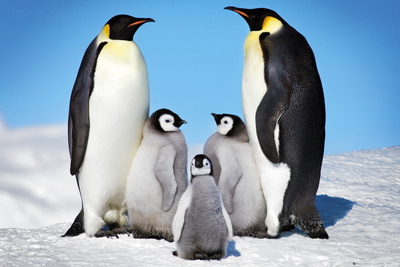
\includegraphics[scale=.50]{figures/Penguins.jpg}
\caption{TAMU figure}
\label{fig:tamu-fig5}
\end{figure}

%%%%%%%%%%%%%%%%%%%%%%%%%%%%%%%%%%%%%%%%%%%%%%%%%%%
%
%  New template code for TAMU Theses and Dissertations starting Fall 2016.
%
%
%  Author: Sean Zachary Roberson 
%	 Version 3.16.09 
%  Last updated 9/12/2016
%
%%%%%%%%%%%%%%%%%%%%%%%%%%%%%%%%%%%%%%%%%%%%%%%%%%%

%%%%%%%%%%%%%%%%%%%%%%%%%%%%%%%%%%%%%%%%%%%%%%%%%%%%%%%%%%%%%%%%%%%%%%
%%                           APPENDIX B
%%%%%%%%%%%%%%%%%%%%%%%%%%%%%%%%%%%%%%%%%%%%%%%%%%%%%%%%%%%%%%%%%%%%%

\chapter{\uppercase {A Second Appendix Whose Title Is Much Longer Than The First}}

Text for the Appendix follows.

\begin{figure}[h]
\centering
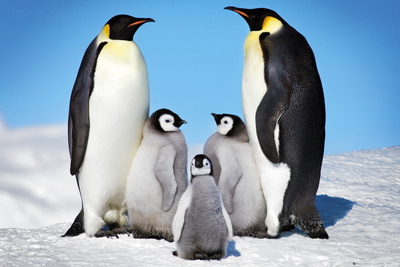
\includegraphics[scale=.50]{figures/Penguins.jpg}
\caption{Another TAMU figure.}
\label{fig:tamu-fig6}
\end{figure}

\section{Appendix Section}

\section{Second Appendix Section}


\pagebreak{}

\end{appendices}


\end{document}
